% 华电毕业论文封面 
\documentclass[UTF8,a4paper]{ctexart}
\usepackage{geometry} % 设置页边距,页面大小
\geometry{left=2.5cm,right=2.0cm,top=2.50cm,bottom=2.0cm}
\linespread{1.3}%调整行间距
\usepackage{graphicx} % 引入图片
\pagestyle{plain}    
\usepackage{setspace} %行间距
\usepackage{array} %
\usepackage{booktabs} %调整表格线与上下内容的间隔
\usepackage{multirow}
\usepackage{hyperref} %加入书签跳转
\usepackage{fontspec} %引入字体Times New Roman字体
%\setmainfont{Times New Roman}             %设置正文字体为Times New Roman
\usepackage{abstract} % 修改摘要


%\usepackage[fontset=windows]{ctex}
\usepackage{xeCJK} %调用系统中已安装的字体
\setCJKmainfont{SimSun}
\setmainfont{Times New Roman}

%% 目录格式设置
\usepackage{tocloft}      %必须这么写,否则会报错
\renewcommand{\contentsname}{\centerline{\Large{\heiti{目\quad\quad 录}}}}
%\renewcommand{\cftchapleader}{\cftdotfill{0.6}} %设置chapter条目的引导点间距
\renewcommand{\cftsecleader}{\cftdotfill{0.6}}
\renewcommand{\cftsubsecleader}{\cftdotfill{0.6}}
\renewcommand{\cftsubsubsecleader}{\cftdotfill{0.6}}
%\renewcommand{\cftchapfont}{\hts}    %设置chapter条目的字体
\renewcommand{\cftsecfont}{\heiti}    %设置section条目的字体
\renewcommand{\cftsecfont}{\Large}    %设置section条目的四号
\renewcommand{\cftsubsecfont}{\songti} %设置subsection条目的字体
\renewcommand{\cftsubsecfont}{\large} %设置subsection条目的字体
\renewcommand{\cftsubsubsecfont}{\songti} %设置subsection条目的字体
\renewcommand{\cftsubsubsecfont}{\large} %设置subsection条目的字体

% 插入代码块
\usepackage{listings}
\usepackage{xcolor}
\lstset{
 %language=bash,                % the language of the code
 columns=fixed,       
% numbers=left,                                        % 在左侧显示行号
% numberstyle=\tiny\color{gray},                       % 设定行号格式
 frame=none,                                          % 不显示背景边框
 backgroundcolor=\color[RGB]{245,245,244},            % 设定背景颜色
 keywordstyle=\color[RGB]{40,40,255},                 % 设定关键字颜色
 numberstyle=\footnotesize\color{darkgray},           
 commentstyle=\it\color[RGB]{0,96,96},                % 设置代码注释的格式
% stringstyle=\rmfamily\slshape\color[RGB]{128,0,0},   % 设置字符串格式
}


% 参考文献
\usepackage{cite}
%%%%%%%%%%%%%%%%%%%%%%%%%%%%%%%%%%%%%%%%%%%%%%%%%%%%%%%%%%%%%%%%%%%%%%%%%%%%%%%%%
%  正文
\begin{document}
%% 封面
% 这是封面
\begin{flushright}
\end{flushright}
\begin{center}
    \vskip 1.5cm
    
\includegraphics[scale=0.6]{figs/ncepu.eps}%学校图标
\end{center}
\begin{center}
    \vskip 1.5cm
    
\includegraphics[scale=0.6]{figs/bthesistitle.eps}%毕业设计图标
\end{center}
\begin{center}
  \vskip 2cm
    \fontsize{15}{1} \textbf{题目} \underline{基于Qemu模拟器移植rCore操作系统的开发与实现}
  \vskip 2.5cm
\end{center}
\begin{center}
  \begin{tabular}{l}

    院\quad\quad 系 \underline{\qquad 控制与计算机工程学院 \quad }\\\\
    专\quad\quad 业 \underline{\qquad 计算机科学与技术 \quad\qquad}\\\\
    % \quad 代表空格,输入题目后自己调长度
    班\quad\quad 级 \underline{\qquad\quad 计算1702班 \quad\qquad\quad }\\\\
    学生姓名 \underline{\qquad\qquad 杨秉学\qquad\qquad\qquad}\\\\
    学\quad\quad 号 \underline{\qquad\quad 120171080212 \qquad\qquad }\\\\
    指导教师 \underline{\qquad\qquad\quad 琚贇\qquad\qquad\qquad }\\\\

  \end{tabular}
\end{center}
\begin{center}
        \vskip 2.5cm
    {2021} 年{\quad 六\quad }月{\qquad \qquad }日

\end{center}
\thispagestyle{empty} %去除本页页码
      
%%摘要
%%%% 中文摘要
% 这是中文摘要
\newpage
\pagenumbering{Roman}
\renewcommand{\abstractname}{\heiti{\Large{摘\quad \quad \quad \quad 要}}}
\begin{abstract}
\addcontentsline{toc}{section}{\heiti{\Large{摘 \quad \quad 要}}}    
{\large{RISC-V是一款近年来最为流行的开源指令集架构,被广泛应用于各个场景。Linux也是一个十分流行的开源操作系统内核。本实验采取Qemu虚拟化技术模拟RISC-V指令环境,解决跨平台的模型部署和运行问题。在上面进行移植Linux操作系统,尝试在上面编译安装程序,并对RISC-V指令集以及操作系统,计算机组成原理,计算机体系结构综合知识进行回顾与总结。}}

%\\ \hspace*{\fill} \\  %换行,用空格填充,再换行,即可实现空出一整行的效果,不需任何环境调整
\noindent %取消首航缩进
    {\large{\textbf{关键字}:RISC-V;Qemu;linux;系统移植;}}
\end{abstract}

%%%% 英文摘要
% 这是英文摘要
\newpage
\renewcommand{\abstractname}{\Large \textbf{ABSTRACT}}
\begin{abstract}
{\large{This section is where the summary information is placed.This section is where the summary information is placed.This section is where the summary information is placed.}}

\noindent
\textbf{KEY WORDS:}RISC-V,Qemu,linux
\end{abstract}

%% 目录
\newpage
\tableofcontents
\thispagestyle{empty}

%% 章节
\newpage
\pagenumbering{arabic}
%%%%定制标题样式
%%%%% section
\CTEXsetup[name={第,章 },format={\centering\heiti\zihao{-2}},aftername={\enspace},beforeskip={24bp},afterskip={18bp}]{section} %name选项中不要使用中文逗号 \zihao(-2)字号小二
%%%%% subsection
\CTEXsetup[format={\raggedright\songti\zihao{-3}},aftername={\enspace},beforeskip={24bp},afterskip={6bp}]{subsection}
%%%%% subsubsection
\CTEXsetup[format={\raggedright\songti\zihao{4}},aftername={\enspace},beforeskip={12bp},afterskip={6bp}]{subsubsection}

% 本章节是介绍项目的背景信息
\section{背景}
在“中兴事件”刚过没多久,某国家就开始发起“华为事件”,对我国半导体产业的打击极大,放眼整个产业链,我们国家连一个像样的指令集架构都没有,我们想研究开发产品竟然还需要别人来授权,这是莫大的耻辱。
所以,我觉得是时候我应该研究一下了。
Risc-v是一个最近流行基于RISC指令集架构,类似与软件领域开源的linux一样,Risc-V也有很多领域可以发挥作用。

  % 介绍背景
% 本章节是介绍意义的
\section{意义}
虽然,已经国内已经有人做出了基于RISC-V处理器内核,linus也把riscv-linux合并到Linux的主分支上了,但是我在这个毕设的过程中复习了一下本科学得全部知识,这为我日后的发展打下了坚实的基础。


% 意义
% 本章节介绍RISC-V的原理
\section{Risc-V模拟器原理}
\subsection{KVM \& Qemu}
首先Qemu(Quick Emulator)本身并不完全是KVM的一部分,它是一套由软件模拟实现的。

而KVM(Kernel Virtual Machine)是有两部分组成,一部分是Linux内核的KVM模块,另一块是经过简化后的Qemu。它能够让Linux主机成为一个Hypervisor(虚拟机监控器)。在支持VMX(Virtual    Machine Extension)功能的x86处理器中,Linux在原有的用户模式和内核模式中新增加了客户模式,并且客户模式也拥有自己的内核模式和用户模式,虚拟机就是运行在客户模式中。三层结构如   图\ref{fig:kvm}

\begin{figure}[htbp]
  \centering %居中显示
  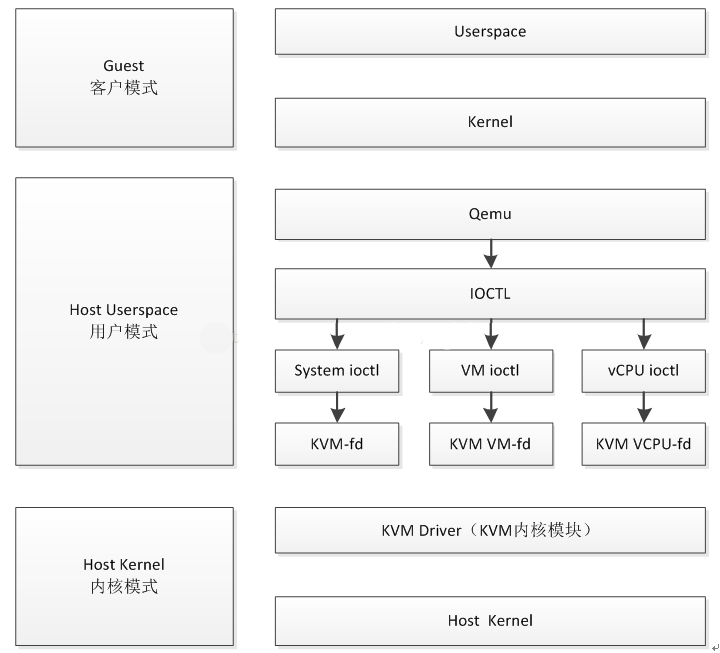
\includegraphics[width=0.6 \textwidth]{figs/KVM三种模式的层次关系.png}
  \caption{KVM三种模式的层次关系}
  \label{fig:kvm} %设置图形引用名称
\end{figure}
%『h』当前位置。将图形放置在正文文本中给出该图形环境的地方。如果本页所剩的页面不够,这一参数将不起作用。
%『t』顶部。将图形放置在页面的顶部。
%『b』底部。将图形放置在页面的底部。
%『p』浮动页。将图形放置在一只允许有浮动对象的页面上。
 %介绍RISC-V模拟器的原理
% 本章节是介绍实验流程
\section{实验流程}
本实验是参考Github上的项目 \cite{BusyBear} 来实现的。

\subsection{实验平台}
本实验环境是在 x86 平台,基于linux环境进行的,具体信息如图\ref{fig:gentoo} 

\begin{figure}[htbp]
  \centering %居中显示
  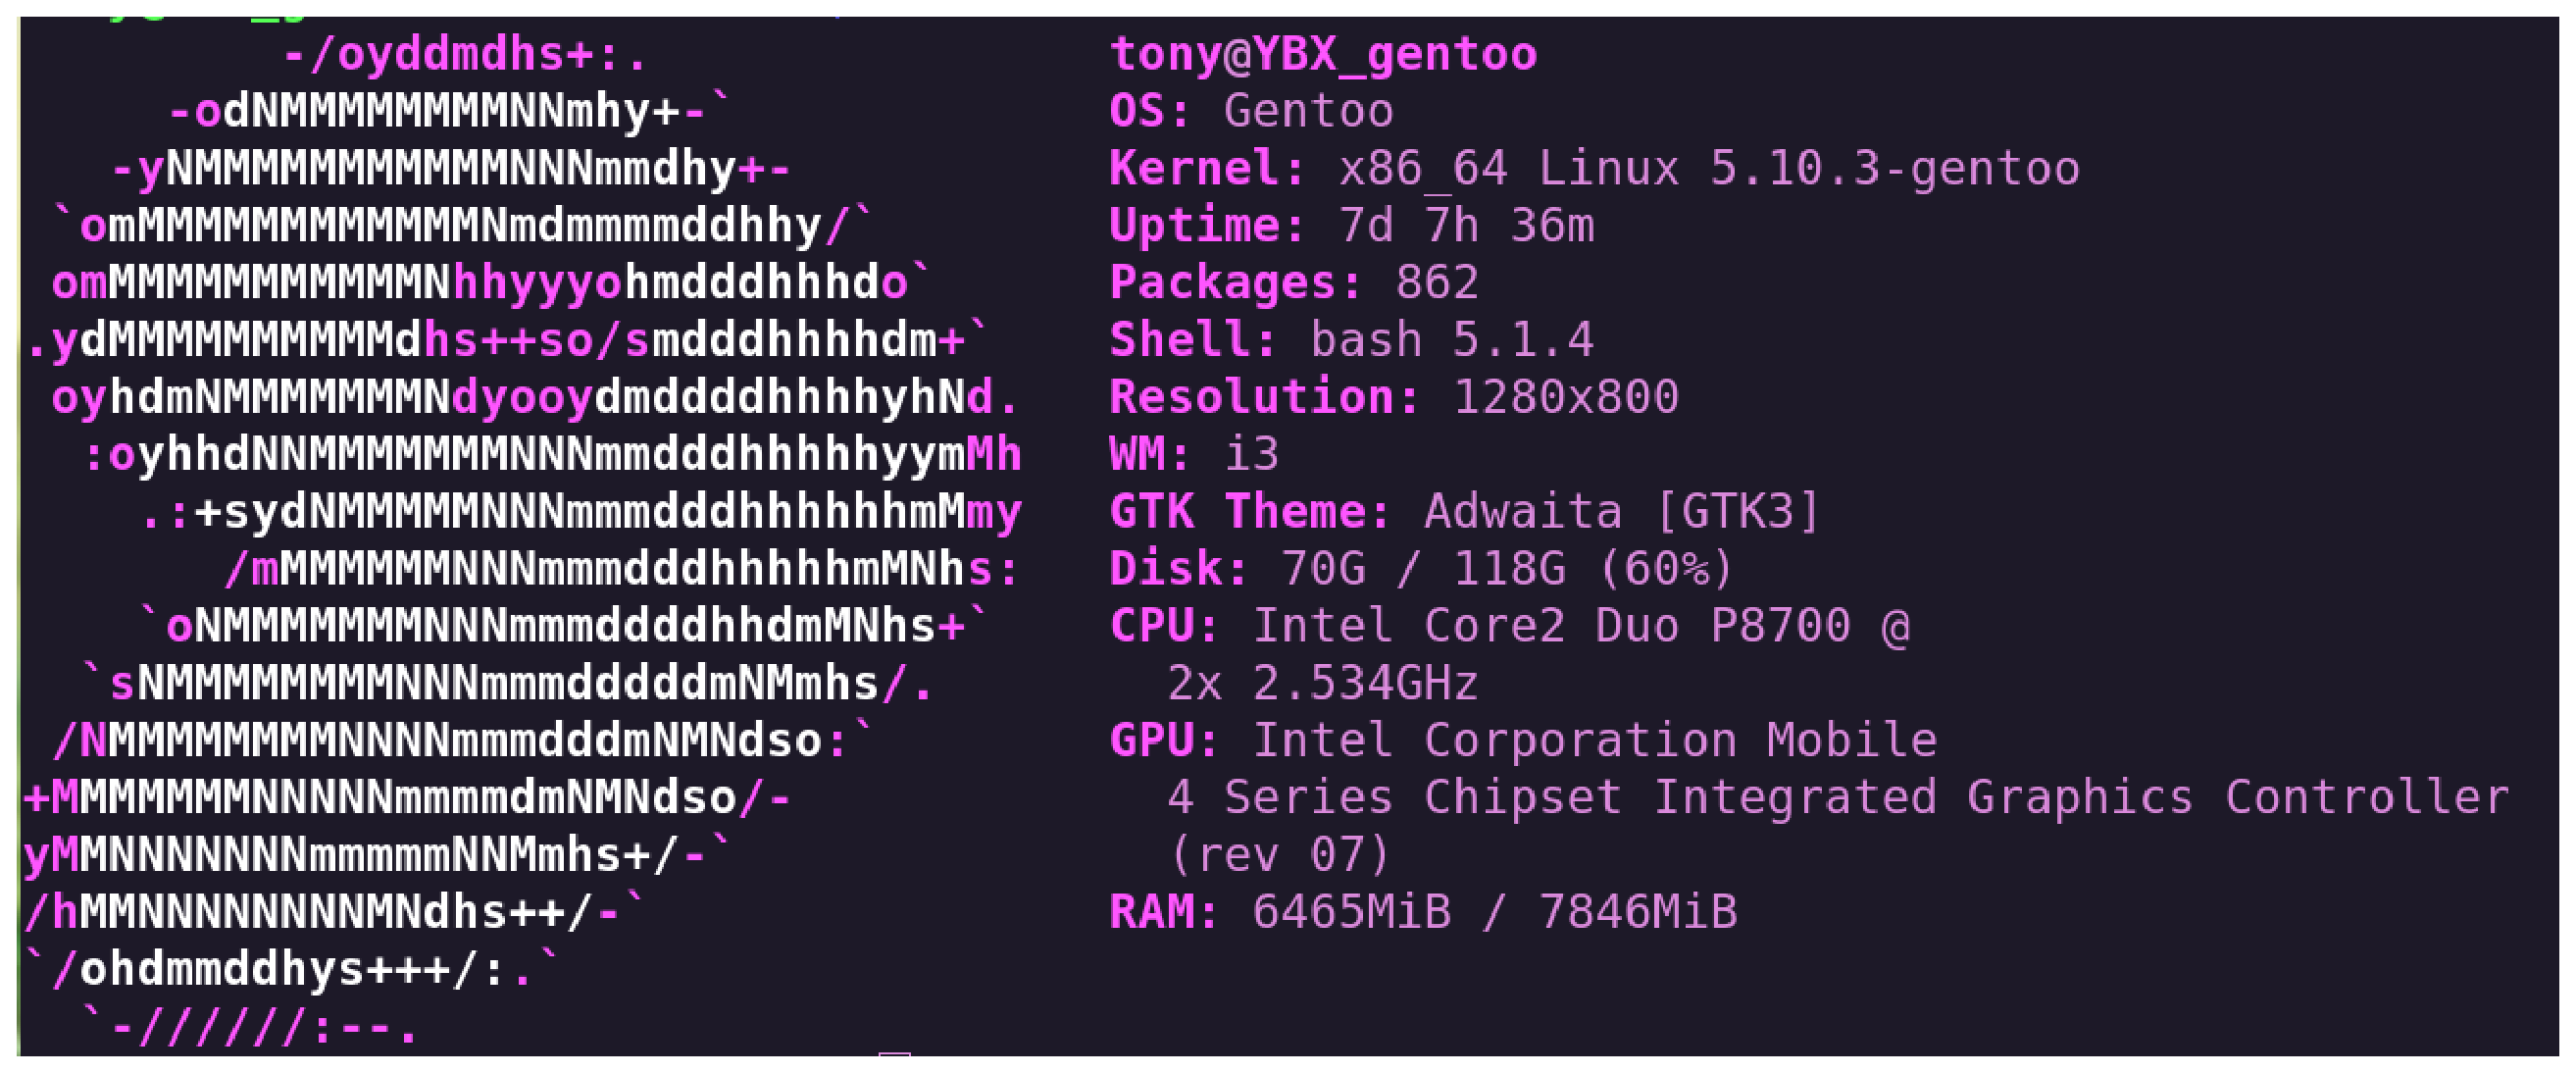
\includegraphics[width=0.6 \textwidth]{figs/gentoo_Logo.eps}
  \caption{实验操作系统}
  \label{fig:gentoo} %设置图形引用名称
\end{figure}

\subsection{Qemu搭建}
在 Gentoo 官方的 Wiki 手册中可以参考 \cite{GentooQemu}
\subsubsection{检测处理器是否支持虚拟化}
\begin{lstlisting}
\$ grep --color -E "vmx|svm" /proc/cpuinfo 
\end{lstlisting}
如果能显示出 图\ref{fig:vmx_svm} 说明处理器是支持虚拟化的

\begin{figure}[htbp]
  \centering %居中显示
  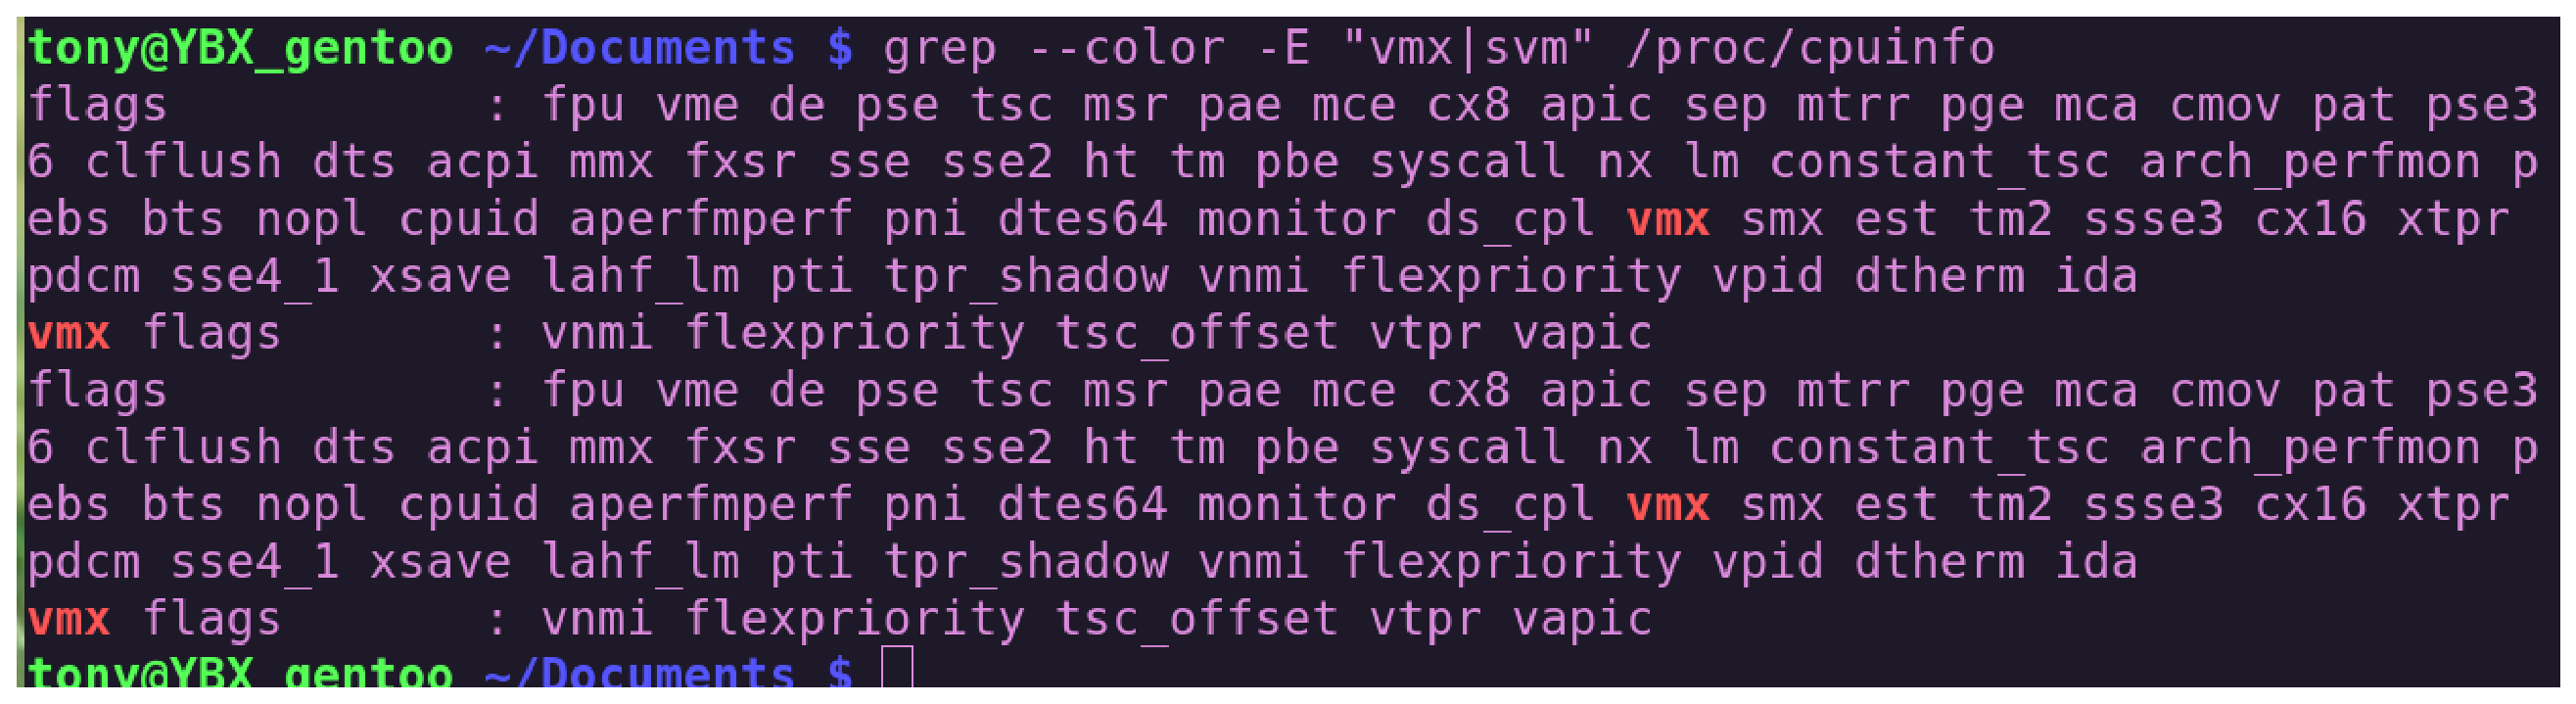
\includegraphics[width=0.6 \textwidth]{figs/vmx_svm.eps}
  \caption{是否支持虚拟化}
  \label{fig:vmx_svm} %设置图形引用名称
\end{figure}

\subsubsection{编译内核}
首先需要更改内核配置

\begin{lstlisting}
cd /usr/src/linux
make menuconfig 
\end{lstlisting}

然后根据以下步骤进行配置内核,使其支持KVM,其中 图\ref{fig:KVM_Intel} 是根据自己处理器来选择的,我的是Intel的处理器,如果使用AMD处理器的话,需要勾选另一个。

\begin{figure}[htbp]
  \centering %居中显示
  \includegraphics[width=0.9 \textwidth]{figs/Kernel/Step1.eps}
  \caption{Virtualization}
  \label{fig:Virtualization} %设置图形引用名称
\end{figure}

\begin{figure}[htbp]
  \centering %居中显示
  \includegraphics[width=0.9 \textwidth]{figs/Kernel/Step2.eps}
  \caption{Kernel-based Virtual Machine (KVM) support}
  \label{fig:Kernel-based} %设置图形引用名称
\end{figure}

\begin{figure}[htbp]
  \centering %居中显示
  \includegraphics[width=0.9 \textwidth]{figs/Kernel/Step3.eps}
  \caption{KVM for Intel processors support}
  \label{fig:KVM_Intel} %设置图形引用名称
\end{figure}

\subsubsection{修改USE Flags并安装}
\begin{lstlisting}
# vim /etc/portage/make.conf
QEMU_SOFTMMU_TARGETS="riscv32 risc64"
QEMU_USER_TARGETS="x86_64"

# vim /etc/portage/package.use
app-emulation/qemu qemu_softmmu_targets_arm qemu_softmmu_targets_x86_64 qemu_softmmu_targets_sparc
app-emulation/qemu qemu_user_targets_x86_64

% 进行安装
# emerge --ask app-emulation/qemu -y
\end{lstlisting}

\subsection{简便方法}
这个步骤是比较偷懒的方式,你可以直接下载网上已经提供编译好而且运行没问题的二进制包,直接运行,但是我下载了,就没运行成功,所以就没有截图演示。
\begin{lstlisting}
cd release
wget https://github.com/michaeljclark/busybear-linux/releases/download/v1.0/bbl.bz2
wget https://github.com/michaeljclark/busybear-linux/releases/download/v1.0/busybear.bin.bz2
bzip2 -d *.bz2
\end{lstlisting}

\subsection{安装GNU工具链}

\begin{lstlisting}
mkdir YBX-bishe
cd YBX-bishe/
# 拉取 gnu-toolchain
git clone --recursive https://github.com/riscv/riscv-gnu-toolchain

# 编译生成 RISC-V newlib & Linux toolchains
cd riscv-gnu-toolchain
./configure --prefix=/opt/riscv --enable-multilib
make newlib -j5
make linux -j5
export PATH=$PATH:/opt/riscv/bin
export RISCV=/opt/risc
$
\end{lstlisting}

\subsection{创建根文件系统}
\begin{lstlisting}
cd ..
git clone https://github.com/michaeljclark/busybear-linux.git
cd busybear-linux
make -j5
\end{lstlisting}

但是这没完,因为busybear会自动帮你下载好 busybox 但是需要自己进行解压和编译

\begin{lstlisting}
CROSS_COMPILE=riscv{{bits}}-unknown-linux-gnu- make menuconfig
CROSS_COMPILE=riscv{{bits}}-unknown-linux-gnu- make
\end{lstlisting}

下面咱们就要制做最小文件系统
\begin{lstlisting}
qemu-img create rootfs.img  1g
mkfs.ext4 rootfs.img
mkdir rootfs
sudo mount -o loop rootfs.img  rootfs
cd rootfs
sudo cp -r ../busyboxsource/_install/* .
sudo mkdir proc sys dev etc etc/init.d
cd etc/init.d/
sudo touch rcS
sudo vi rcS
#!/bin/sh
mount -t proc none /proc
mount -t sysfs none /sys
/sbin/mdev -s

sudo mod +x rcS
sudo umount rootfs
\end{lstlisting}

\subsection{构建Linux内核}
\begin{lstlisting}
git clone https://github.com/torvalds/linux
cd linux
git checkout v5.4
make ARCH=riscv CROSS_COMPILE=riscv64-unknown-linux-gnu- defconfig
make ARCH=riscv CROSS_COMPILE=riscv64-unknown-linux-gnu-
\end{lstlisting}

\subsection{制作BootLoader——BBL(Berkeley Boot Loader)}
\begin{lstlisting}
cd..
git clone https://github.com/riscv/riscv-pk.git
cd riscv-pk
mkdir build
cd build
../configure --enable-logo --host=riscv64-unknown-elf --with-payload=../../riscv-linux/vmlinux
make -j8
\end{lstlisting}

\subsection{运行}
\begin{lstlisting}
cd ..
mkdir Running
cd Running
\end{lstlisting}
创建KVM启动脚本
\begin{lstlisting}
vim open_kvm
#!/bin/sh
sudo /etc/init.d/libvirtd start
sudo virsh net-start default  #开启网络服务
\end{lstlisting}

创建KVM关闭脚本
\begin{lstlisting}
sudo virsh net-destory default
sudo /etc/init.d/libvirtd stop
\end{lstlisting}


创建网络启动脚本
\begin{lstlisting}
#!/bin/sh
brctl addif virbr0 $1
ifconfig $1 up
\end{lstlisting}

创建网络关闭脚本
\begin{lstlisting}
#!/bin/sh
ifconfig $1 down
brctl delif virbr0 $1
\end{lstlisting}

创建程序运行脚本
\begin{lstlisting}
#!/bin/sh
# QEMU 5.2以后.模拟器内部集成了OpenSBI
sudo qemu-system-riscv64 \
  -nographic -machine virt \
  -m 1024M \
  -kernel bbl \
  -kernel /home/tony/Documents/Risc-v/busybear-linux/build/linux-5.0/arch/riscv/boot/Image \
  -drive file=busybear.bin,format=raw,id=hd0 \
  -device virtio-blk-device,drive=hd0 \
  -device virtio-net-device,netdev=net0 \
  -netdev type=tap,script=./ifup.sh,downscript=./ifdown.sh,id=net0 \
  -append "root=/dev/vda ro console=ttyS0" 
\end{lstlisting}






\subsection{最终效果}
最终结果演示可以看 \cite{结果演示} 



 % 介绍实验过程
% 本章节介绍与前人的比较
\section{与前人比较}
  %与前人比较


根据 David A. Patterson 的著作\cite{2006Computer}

%% 参考文献
\bibliographystyle{plain}
\bibliography{Ref}
%\bibliographystyle{plain}指定参考文献的呈现方式,常见的预设样式的可选项有8种,分别是:
%% 1. plain,按字母的顺序排列,比较次序为作者、年度和标题;
%% 2. unsrt,样式同plain,只是按照引用的先后排序;
%% 3. alpha,用作者名首字母+年份后两位作标号,以字母顺序排序;
%% 4. abbrv,类似plain,将月份全拼改为缩写,更显紧凑;
%% 5. ieeetr,国际电气电子工程师协会期刊样式;
%% 6. acm,美国计算机学会期刊样式;
%% 7. siam,美国工业和应用数学学会期刊样式;
%% 8. apalike,美国心理学学会期刊样式;
\end{document}
